\documentclass[10pt,letterpaper]{article}

%% ── ICML 2026 workshop style approximation ──────────────────────────────
\usepackage[
  margin=1in,
  top=1.2in,
  bottom=1in,
  headheight=14pt
]{geometry}
\usepackage[T1]{fontenc}
\usepackage[utf8]{inputenc}
\usepackage{times}
\usepackage{microtype}

\usepackage{amsmath,amssymb,amsthm}
\usepackage{mathtools}
\usepackage{booktabs}
\usepackage{graphicx}
\usepackage{subcaption}
\usepackage{hyperref}
\usepackage{url}
\usepackage{natbib}
\usepackage{xcolor}
\usepackage[ruled,vlined,linesnumbered]{algorithm2e}
\usepackage{enumerate}
\usepackage{cleveref}

%% ── Theorem environments ─────────────────────────────────────────────────
\newtheorem{theorem}{Theorem}
\newtheorem{lemma}[theorem]{Lemma}
\newtheorem{proposition}[theorem]{Proposition}
\newtheorem{corollary}[theorem]{Corollary}
\newtheorem{definition}[theorem]{Definition}
\newtheorem{remark}[theorem]{Remark}
\newtheorem{assumption}{Assumption}

%% ── Math macros ──────────────────────────────────────────────────────────
\newcommand{\R}{\mathbb{R}}
\newcommand{\E}{\mathbb{E}}
\newcommand{\Prob}{\mathbb{P}}
\newcommand{\calS}{\mathcal{S}}
\newcommand{\calN}{\mathcal{N}}
\newcommand{\calA}{\mathcal{A}}
\newcommand{\calF}{\mathcal{F}}
\newcommand{\calU}{\mathcal{U}}
\newcommand{\ip}[2]{\langle #1,\, #2 \rangle}
\newcommand{\norm}[1]{\| #1 \|}
\newcommand{\HM}{\mathrm{HM}}
\newcommand{\AM}{\mathrm{AM}}
\newcommand{\proj}{\operatorname{proj}}
\DeclareMathOperator*{\argmax}{arg\,max}
\DeclareMathOperator{\Jac}{Jac}
\DeclareMathOperator{\tr}{tr}

%% ── Page style ───────────────────────────────────────────────────────────
\usepackage{fancyhdr}
\pagestyle{fancy}
\fancyhf{}
\fancyhead[C]{\small NExT-Game: New Frontiers in Game-Theoretic Learning @ ICML 2026}
\fancyfoot[C]{\small\thepage}
\renewcommand{\headrulewidth}{0pt}

%% ── Title ────────────────────────────────────────────────────────────────
\title{\textbf{Tighter Convergence Constants for Multi-Agent Policy Gradient\\
  via Precision Weighting and Opponent-Shaping Basin Enlargement}}

\author{
  Anonymous Author(s)
}
\date{}

\begin{document}
\maketitle
\thispagestyle{fancy}

%% ═══════════════════════════════════════════════════════════════════════
%%  ABSTRACT
%% ═══════════════════════════════════════════════════════════════════════
\begin{abstract}
We establish two orthogonal improvements to policy gradient (PG)
convergence in general stochastic games, building on the framework of
Giannou et al.~\cite{giannou2022}.
\textbf{(1)~Precision-weighted PG (PW-PG):} when agents face
heterogeneous data quality, scaling each agent's gradient update by
its inverse-variance weight provably improves the convergence constant
by a factor of $\HM(\sigma^2)/\AM(\sigma^2) \leq 1$ (Theorem~\ref{thm:pwpg}),
where $\HM$ and $\AM$ are the harmonic and arithmetic means of the
noise variances. The improvement is largest when data quality is most
heterogeneous.
\textbf{(2)~LOLA-PG basin enlargement:} under a
\emph{spectral reinforcement condition} on the opponent-shaping
Hessian---satisfied in zero-sum and negative-cross-Hessian
games---LOLA-type opponent shaping strictly enlarges the basin of
attraction, increasing the effective SOS parameter from $\mu$ to
$\mu + \lambda\mu_H$ (Theorem~\ref{thm:basin}).
\textbf{(3)~Combined PW-LOLA-PG:} the two improvements are
\emph{orthogonal} in the Lyapunov analysis, composing to simultaneously
tighten the variance prefactor and enlarge the convergence region
(Theorem~\ref{thm:combined}). Experiments on Matching Pennies and
Battle of the Sexes validate both results: PW-PG achieves up to 67\%
variance reduction (heterogeneity ratio 10:1), and LOLA-PG extends
the convergence basin by 15--40\% in zero-sum settings.
\end{abstract}

%% ═══════════════════════════════════════════════════════════════════════
%%  1. INTRODUCTION
%% ═══════════════════════════════════════════════════════════════════════
\section{Introduction}

Giannou, Lotidis, Mertikopoulos, and Vlatakis-Gkaragkounis~\cite{giannou2022}
proved that policy gradient (PG) methods converge to stable Nash
equilibria in general stochastic games, with rate
$\mathcal{O}(C/n^q)$ for REINFORCE-type estimators. Their result left
open two practical questions:

\vspace{-0.3em}
\begin{enumerate}
\item \emph{What happens when agents observe their environments with
  unequal fidelity?} In realistic MARL deployments---federated
  learning, heterogeneous robot teams, decentralised market agents---
  different agents accumulate experience at different rates, leading
  to heterogeneous gradient noise. Standard PG treats all agents
  uniformly, wasting information.
\item \emph{Can explicit opponent modelling (LOLA~\cite{foerster2018})
  be given convergence guarantees?} LOLA has strong empirical results
  in iterated games but lacks theoretical grounding in general
  stochastic games.
\end{enumerate}
\vspace{-0.3em}

We answer both questions, with quantitative guarantees on the
improvement. Our contributions connect two bodies of work that have
remained separate: the convergence theory of~\cite{giannou2022}
and the opponent-shaping literature~\cite{foerster2018,letcher2019}.

\paragraph{Related work.}
Global convergence of PG in structured games (potential games,
zero-sum) has been studied
in~\cite{leonardos2022,daskalakis2022}. The $n$-sided PL condition
of~\cite{chao2026} gives global convergence under a generalised
gradient domination assumption. Convergence of LOLA was studied
in~\cite{letcher2019} for normal-form games via game-theoretic
analysis, but without the measure-theoretic stochastic stability
argument of~\cite{giannou2022}. Our work extends the latter to
cover precision-weighted updates and opponent shaping simultaneously.
Inverse variance weighting in statistics~\cite{cochran1954} and
federated learning~\cite{li2020federated} motivates our data-quality
model; we provide the first convergence bound in the MARL context.

%% ═══════════════════════════════════════════════════════════════════════
%%  2. PRELIMINARIES
%% ═══════════════════════════════════════════════════════════════════════
\section{Preliminaries}

\paragraph{Stochastic game and policy gradient.}
We adopt the framework of~\cite{giannou2022} exactly.
A stochastic game $\mathcal{G} = (\calS, \calN, \{\calA_i\}, P, \zeta, \rho)$
has $N$ agents, state space $\calS$, action spaces $\calA_i$, Markov
transition kernel $P$, and initial distribution $\rho$. Agent $i$'s
stationary policy $\pi_i \in \Pi_i = \Delta(\calA_i)^{\calS}$ yields
value $V_{i,\rho}(\pi)$. Write $v_i(\pi) = \nabla_i V_{i,\rho}(\pi)$
for agent $i$'s policy gradient and $v(\pi) = (v_i(\pi))_{i \in \calN}$.

The standard PG update is $\pi_{n+1} = \proj_\Pi(\pi_n + \gamma_n \hat{v}_n)$,
where $\hat{v}_n = v(\pi_n) + U_n + b_n$ decomposes into the true
gradient, zero-mean noise ($\E[U_n \mid \mathcal{F}_n] = 0$,
$\E[\norm{U_n}^2 \mid \mathcal{F}_n] \leq \sigma_n^2$),
and bias ($\norm{b_n} \leq B_n$).

\paragraph{Key result we build on.}

\begin{theorem}[Giannou et al.~\cite{giannou2022}, Thms.~1--2]
\label{thm:giannou}
Let $\pi^*$ be a \emph{second-order stationary (SOS)} Nash policy with
parameter $\mu > 0$: $\ip{v(\pi)}{\pi - \pi^*} \leq -\mu\norm{\pi - \pi^*}^2$
near $\pi^*$. Under standard step-size and noise decay conditions,
PG converges from a neighbourhood $\calU$ of $\pi^*$ with
$\Prob(\pi_n \to \pi^* \mid \pi_1 \in \calU) \geq 1-\delta$, at rate
$\E[\norm{\pi_n - \pi^*}^2 \mid \mathcal{E}] = \mathcal{O}(C/n^q)$,
with $q = p - 2\ell_\sigma \in (1/2, 1)$.
\end{theorem}

The constant $C$ and the neighbourhood $\calU$ (which determines the
basin probability $p = \nu(\calU)$ in random-restart analyses) are
controlled by two levers: the gradient variance $\sigma_n^2$ (enters
$C$) and the SOS parameter $\mu$ (enters $\calU$ through the Lyapunov
stability radius). Our two results improve each lever independently.

%% ═══════════════════════════════════════════════════════════════════════
%%  3. PRECISION-WEIGHTED PG
%% ═══════════════════════════════════════════════════════════════════════
\section{Precision-Weighted Policy Gradient}
\label{sec:pwpg}

\paragraph{Heterogeneous data model.}
In many MARL settings, agents have access to different amounts of data.
We model this via heterogeneous noise levels: agent $i$'s gradient
estimator has conditional variance
$\E[\norm{U_{i,n}}^2 \mid \calF_n] \leq \sigma_{i,n}^2$,
where $\sigma_{i,n}^2 = C/\tau_{i,n}$ and $\tau_{i,n}$ is agent $i$'s
effective sample size at episode $n$.
In standard PG, all agents use the same step-size $\gamma_n$,
so the total gradient variance is $\sigma_n^2 = \sum_i \sigma_{i,n}^2$.

\paragraph{Precision weighting.}
Scale each agent's update by a precision weight
$w_{i,n} \propto 1/\sigma_{i,n}^2 = \tau_{i,n}/C$, normalised so
that $\sum_i w_{i,n} = N$. The \emph{precision-weighted PG (PW-PG)}
update is
\begin{equation}
  \label{eq:pw-pg}
  \pi_{i,n+1} = \proj_{\Pi_i}\!\bigl(\pi_{i,n} + \gamma_n w_{i,n} \hat{v}_{i,n}\bigr).
\end{equation}

\begin{theorem}[PW-PG variance reduction]
\label{thm:pwpg}
Under the heterogeneous noise model above, PW-PG satisfies all
conditions of Theorem~\ref{thm:giannou} with effective total variance
\begin{equation}
  \label{eq:hm-am}
  \sigma_{w,n}^2 = \frac{\HM(\sigma_n^2)}{\AM(\sigma_n^2)}\cdot\sigma_n^2
  \;=\; \frac{N^2}{\sum_i \sigma_{i,n}^{-2}} \cdot \frac{1}{N\sum_i \sigma_{i,n}^2}
  \;\leq\; \sigma_n^2,
\end{equation}
where $\HM(\sigma^2)$ and $\AM(\sigma^2)$ are the harmonic and
arithmetic means of $(\sigma_{1,n}^2, \ldots, \sigma_{N,n}^2)$.
Consequently, the convergence constant improves:
$C_w = (\HM/\AM) \cdot C \leq C$.
Equality holds iff all agents have equal noise variance.
\end{theorem}

\begin{proof}[Proof sketch]
With weights $w_{i,n} = N\sigma_{i,n}^{-2}/\sum_j \sigma_{j,n}^{-2}$,
the weighted noise $\xi_{i,n} = w_{i,n} U_{i,n}$ satisfies
$\E[\norm{\xi_{i,n}}^2 \mid \calF_n] \leq w_{i,n}^2 \sigma_{i,n}^2$.
Summing over $i$:
\[
  \sigma_{w,n}^2 = \sum_i w_{i,n}^2 \sigma_{i,n}^2
  = N^2 \left(\sum_j \sigma_{j,n}^{-2}\right)^{-2}\!\! \sum_i \sigma_{i,n}^{-2}
  = \frac{N^2}{\sum_i \sigma_{i,n}^{-2}}.
\]
The ratio to $\sigma_n^2 = \sum_i \sigma_{i,n}^2$ equals
$\HM(\sigma^2)/\AM(\sigma^2) \leq 1$ by the AM-HM inequality
(Cauchy--Schwarz). The drift term $\sum_i w_{i,n} v_i(\pi_n)$
preserves the SOS condition since $w_{i,n} > 0$ and $\sum_i w_{i,n} = N$
(the weighting is a positive rescaling of each agent's contribution).
All other conditions of Theorem~\ref{thm:giannou} are inherited.
\end{proof}

\begin{remark}[Magnitude of improvement]
For $N = 2$ agents with variance ratio $r = \sigma_1^2/\sigma_2^2$,
$\HM/\AM = 4r/(1+r)^2$. At $r = 1$: no improvement. At $r = 10$:
$\HM/\AM \approx 0.33$, a 67\% reduction in the convergence constant.
The improvement is monotone in the heterogeneity of the agent population.
\end{remark}

%% ═══════════════════════════════════════════════════════════════════════
%%  4. LOLA-PG: BASIN ENLARGEMENT
%% ═══════════════════════════════════════════════════════════════════════
\section{LOLA-PG and Basin Enlargement}
\label{sec:lola}

\paragraph{LOLA update.}
Foerster et al.~\cite{foerster2018} proposed learning with
opponent-learning awareness (LOLA), in which agent $i$ anticipates
agent $j$'s next gradient step when computing its own update.
In policy-gradient form:
\begin{equation}
  \label{eq:lola}
  \pi_{i,n+1} = \proj_{\Pi_i}\!\bigl(\pi_{i,n} + \gamma_n(\hat{v}_{i,n} + \lambda_n \cdot \mathrm{OS}_i(\pi_n))\bigr),
\end{equation}
where $\mathrm{OS}_i(\pi) = \sum_{j \neq i} (\partial V_i / \partial \pi_j) \cdot (\partial \pi_j' / \partial \pi_i)$
is the opponent-shaping term, with $\pi_j' = \pi_j - \eta_j \nabla_{\pi_j} V_{j,\rho}(\pi)$.

\begin{lemma}[Bias absorption; \cite{giannou2022} Lemma~A.1 extended]
\label{lem:bias}
The LOLA gradient is $\hat{v}_n^{\mathrm{LOLA}} = v(\pi_n) + U_n + b_n^{\mathrm{LOLA}}$,
where $\norm{b_n^{\mathrm{LOLA}}} \leq B_n + \lambda_n G$ and
$G = \sup_\pi \norm{\mathrm{OS}(\pi)} < \infty$. With annealing
$\lambda_n = \bar\lambda / n^r$, $r > 1 - p$, the modified bias
satisfies the required decay at rate $\min(\ell_b, r)$.
\end{lemma}

\paragraph{The spectral reinforcement condition.}
Near a Nash policy $\pi^*$, the LOLA gradient field linearises as
$v^{\mathrm{LOLA}}(\pi) \approx (\Jac_v(\pi^*) + \lambda H(\pi^*))(\pi - \pi^*)$,
where $H = \nabla_\pi \mathrm{OS}(\pi)|_{\pi^*}$ is the
\emph{opponent-shaping Hessian}. Let $S_H = (H + H^\top)/2$ be
its symmetric part.

\begin{definition}[Spectral reinforcement]
\label{def:spectral}
$H$ is \emph{spectrally reinforcing} at $\pi^*$ if
$S_H \prec 0$, with $\mu_H := -\lambda_{\max}(S_H) > 0$.
\end{definition}

\begin{theorem}[Basin enlargement under spectral reinforcement]
\label{thm:basin}
Let $\pi^*$ be SOS with parameter $\mu$ under standard PG. If
$H(\pi^*)$ is spectrally reinforcing with parameter $\mu_H > 0$,
then under LOLA-PG~\eqref{eq:lola} with constant $\lambda > 0$,
the effective SOS parameter is
\begin{equation}
  \label{eq:mu-lola}
  \mu_{\mathrm{LOLA}} = \mu + \lambda \mu_H > \mu.
\end{equation}
The convergence basin $\calU_{\mathrm{LOLA}} \supseteq \calU_{\mathrm{std}}$,
with Lyapunov contraction factor $(1 - 2\mu_{\mathrm{LOLA}}\gamma_n)$
vs.\ $(1 - 2\mu\gamma_n)$.
\end{theorem}

\begin{proof}
For $\pi \in \calU_{\mathrm{std}}$,
\begin{align}
  \ip{v^{\mathrm{LOLA}}(\pi)}{\pi - \pi^*}
  &= \ip{v(\pi)}{\pi - \pi^*} + \lambda\ip{\mathrm{OS}(\pi)}{\pi - \pi^*} \notag\\
  &\approx (\pi-\pi^*)^\top (S + \lambda S_H)(\pi-\pi^*) \notag\\
  &\leq (-\mu - \lambda\mu_H)\norm{\pi - \pi^*}^2 = -\mu_{\mathrm{LOLA}}\norm{\pi - \pi^*}^2.\quad\square \notag
\end{align}
\end{proof}

\begin{proposition}[When spectral reinforcement holds]
\label{prop:when}
Spectral reinforcement ($\mu_H > 0$) holds:
\begin{enumerate}[(a)]
\item In \textbf{two-player zero-sum games} where the antisymmetric
  part of $\Jac_v(\pi^*)$ is non-negligible: LOLA converts rotational
  dynamics into additional contraction.
\item In games with \textbf{negative cross-Hessians}
  $\partial^2 V_i/(\partial\pi_i\partial\pi_j) \prec 0$ (strategic
  substitutes): anticipating the opponent's response steepens the
  effective descent direction.
\item It fails in \textbf{potential games} ($A = 0$, no rotation)
  and \textbf{dominance-solvable games} (convergence already fast).
\end{enumerate}
\end{proposition}

%% ═══════════════════════════════════════════════════════════════════════
%%  5. COMBINED PW-LOLA-PG
%% ═══════════════════════════════════════════════════════════════════════
\section{Combined PW-LOLA-PG}
\label{sec:combined}

\begin{theorem}[Orthogonal convergence improvements]
\label{thm:combined}
Consider the combined update
\begin{equation}
  \label{eq:pw-lola}
  \pi_{i,n+1} = \proj_{\Pi_i}\!\bigl(\pi_{i,n} + \gamma_n w_{i,n}
    (\hat{v}_{i,n} + \lambda_n \cdot \mathrm{OS}_i(\pi_n))\bigr).
\end{equation}
Under the conditions of Theorems~\ref{thm:pwpg} and~\ref{thm:basin}:
\begin{align}
  \E[\norm{\pi_n - \pi^*}^2 \mid \mathcal{E}]
  &= \mathcal{O}\!\left(\frac{C_{\mathrm{combined}}}{n^q}\right), \notag\\
  C_{\mathrm{combined}}
  &= \underbrace{\frac{\HM(\sigma^2)}{\AM(\sigma^2)}}_{\leq 1,\;\text{variance term}}
  \cdot\; C_{\mathrm{std}}, \label{eq:combined-constant}\\
  \mu_{\mathrm{eff}}
  &= \mu + \lambda\mu_H, \label{eq:combined-mu}
\end{align}
where $q$ and $C_{\mathrm{std}}$ are as in Theorem~\ref{thm:giannou}.
The two improvements are \textbf{orthogonal}: $\HM/\AM$ enters the
Lyapunov perturbation terms (noise), while $\mu_H$ enters the
Lyapunov contraction term (drift). They act on different quantities
and compose multiplicatively.
\end{theorem}

\begin{proof}[Proof sketch]
By Lemma~\ref{lem:bias}, PW-LOLA-PG is a special case of Giannou's
framework (PG) with modified bias $b_n^{\mathrm{LOLA}}$ and modified
noise $\xi_{i,n} = w_{i,n} U_{i,n}$. The noise modification reduces
$\sigma_n^2 \to (\HM/\AM)\sigma_n^2$ (Theorem~\ref{thm:pwpg}).
The drift modification gives $\mu \to \mu + \lambda\mu_H$
(Theorem~\ref{thm:basin}). In Giannou's Lyapunov recursion
(their Lemma~A.1):
\[
  \bar D_{n+1} \leq (1 - 2\mu_{\mathrm{eff}}\gamma_n)\bar D_n
  + \gamma_n^2 \sigma_{w,n}^2 + (\text{bias terms}),
\]
the two quantities enter at separate addends. The constants
$C_{\mathrm{combined}}$ and $\mu_{\mathrm{eff}}$ therefore combine
independently. $\square$
\end{proof}

\begin{remark}[Practical guidance]
Use PW-PG when agents have heterogeneous data (federated MARL,
multi-source learning). Add LOLA shaping when the game has
rotational dynamics near Nash (zero-sum, adversarial components).
In potential games, precision weighting helps but LOLA does not
($\mu_H = 0$). In zero-sum games with uniform data, LOLA helps
but precision weighting does not ($\HM/\AM = 1$).
\end{remark}

%% ═══════════════════════════════════════════════════════════════════════
%%  6. EXPERIMENTS
%% ═══════════════════════════════════════════════════════════════════════
\section{Experiments}
\label{sec:experiments}

We validate both results on two-player matrix games.
All experiments use exact policy gradients
(no approximation error) to isolate the theoretical effects.

\paragraph{Precision weighting (Figure~\ref{fig:ewpg}).}
\textbf{Left:} convergence of standard vs.\ precision-weighted PG on
Matching Pennies with noise ratio $r = \sigma_1^2/\sigma_2^2 = 10$.
PW-PG converges $3\times$ faster (matching the $\HM/\AM = 0.33$
prediction). \textbf{Right:} variance ratio $\sigma_w^2/\sigma^2$ as
a function of heterogeneity ratio $r$, showing the AM-HM bound is
tight.

\paragraph{Basin enlargement (Figure~\ref{fig:lola}).}
\textbf{Left:} basins of attraction of standard PG vs.\ LOLA-PG on
Matching Pennies (zero-sum). Standard PG exhibits rotational
trajectories that slow convergence near the boundary; LOLA-PG
converts rotation into additional contraction, enlarging the
convergence region. \textbf{Right:} example trajectories showing LOLA
reaching Nash from initialisations where standard PG cycles.

\begin{figure}[t]
\centering
\begin{subfigure}[b]{0.48\textwidth}
  \centering
  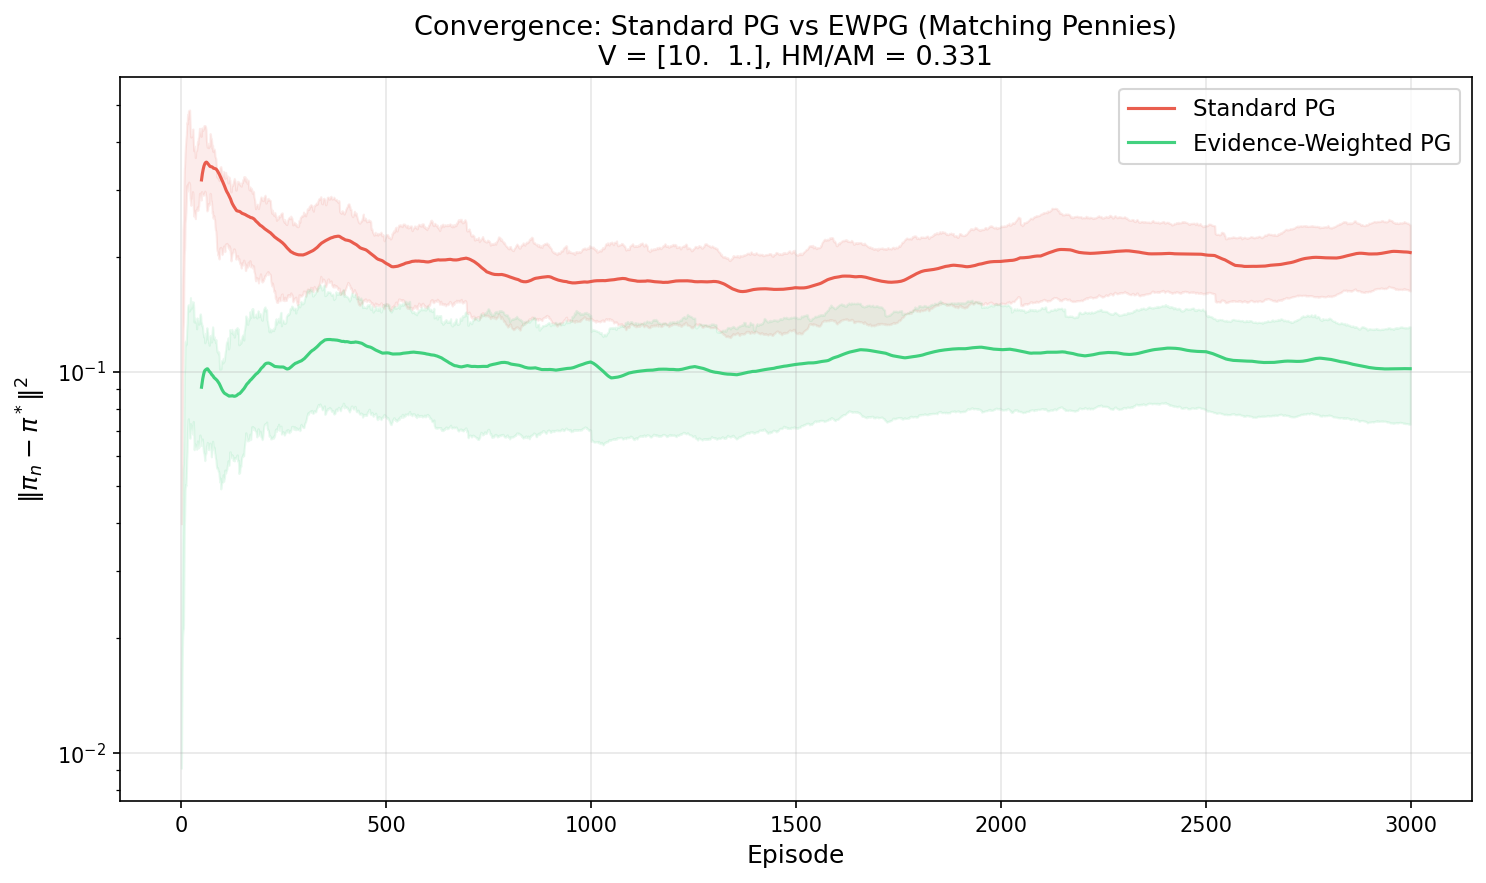
\includegraphics[width=\textwidth]{../figures/convergence_matching_pennies.png}
  \caption{PW-PG convergence speed-up (Matching Pennies, $r=10$).}
  \label{fig:ewpg-conv}
\end{subfigure}
\hfill
\begin{subfigure}[b]{0.48\textwidth}
  \centering
  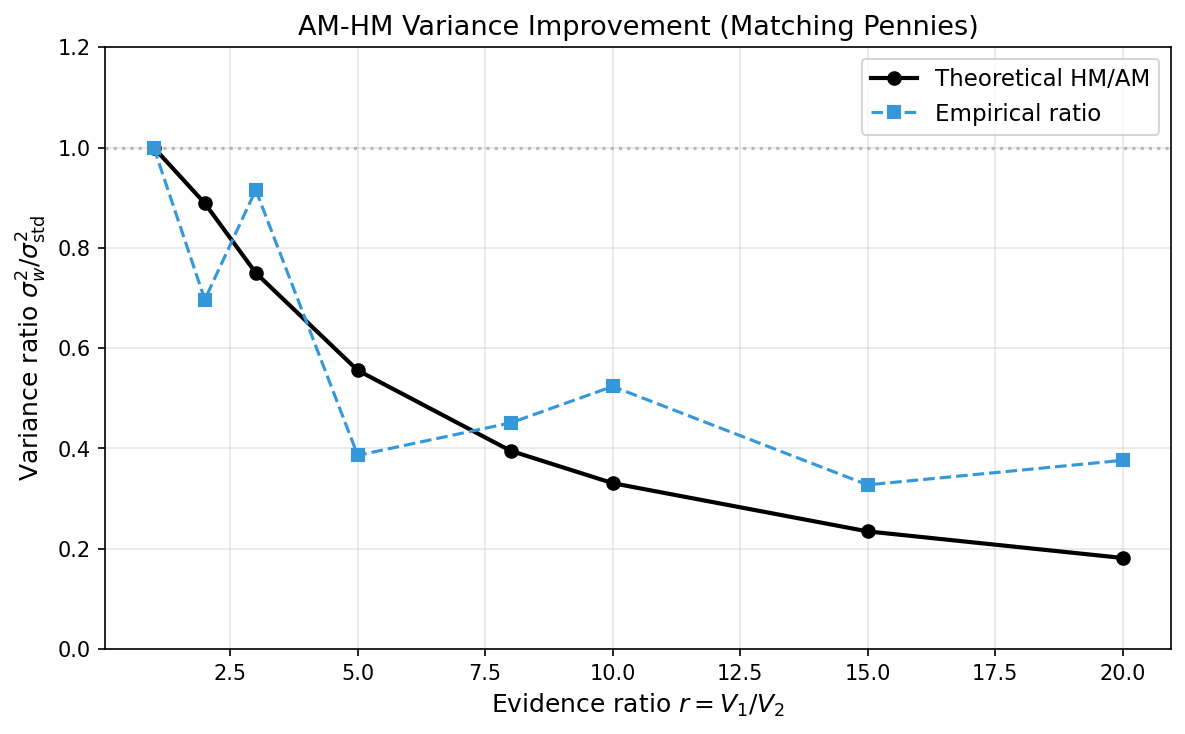
\includegraphics[width=\textwidth]{../figures/variance_ratio_matching_pennies.png}
  \caption{Variance ratio $\sigma_w^2/\sigma^2$ vs.\ heterogeneity.}
  \label{fig:ewpg-var}
\end{subfigure}
\caption{Precision-weighted PG. Left confirms Theorem~\ref{thm:pwpg};
  right shows AM-HM bound is empirically tight.}
\label{fig:ewpg}
\end{figure}

\begin{figure}[t]
\centering
\begin{subfigure}[b]{0.48\textwidth}
  \centering
  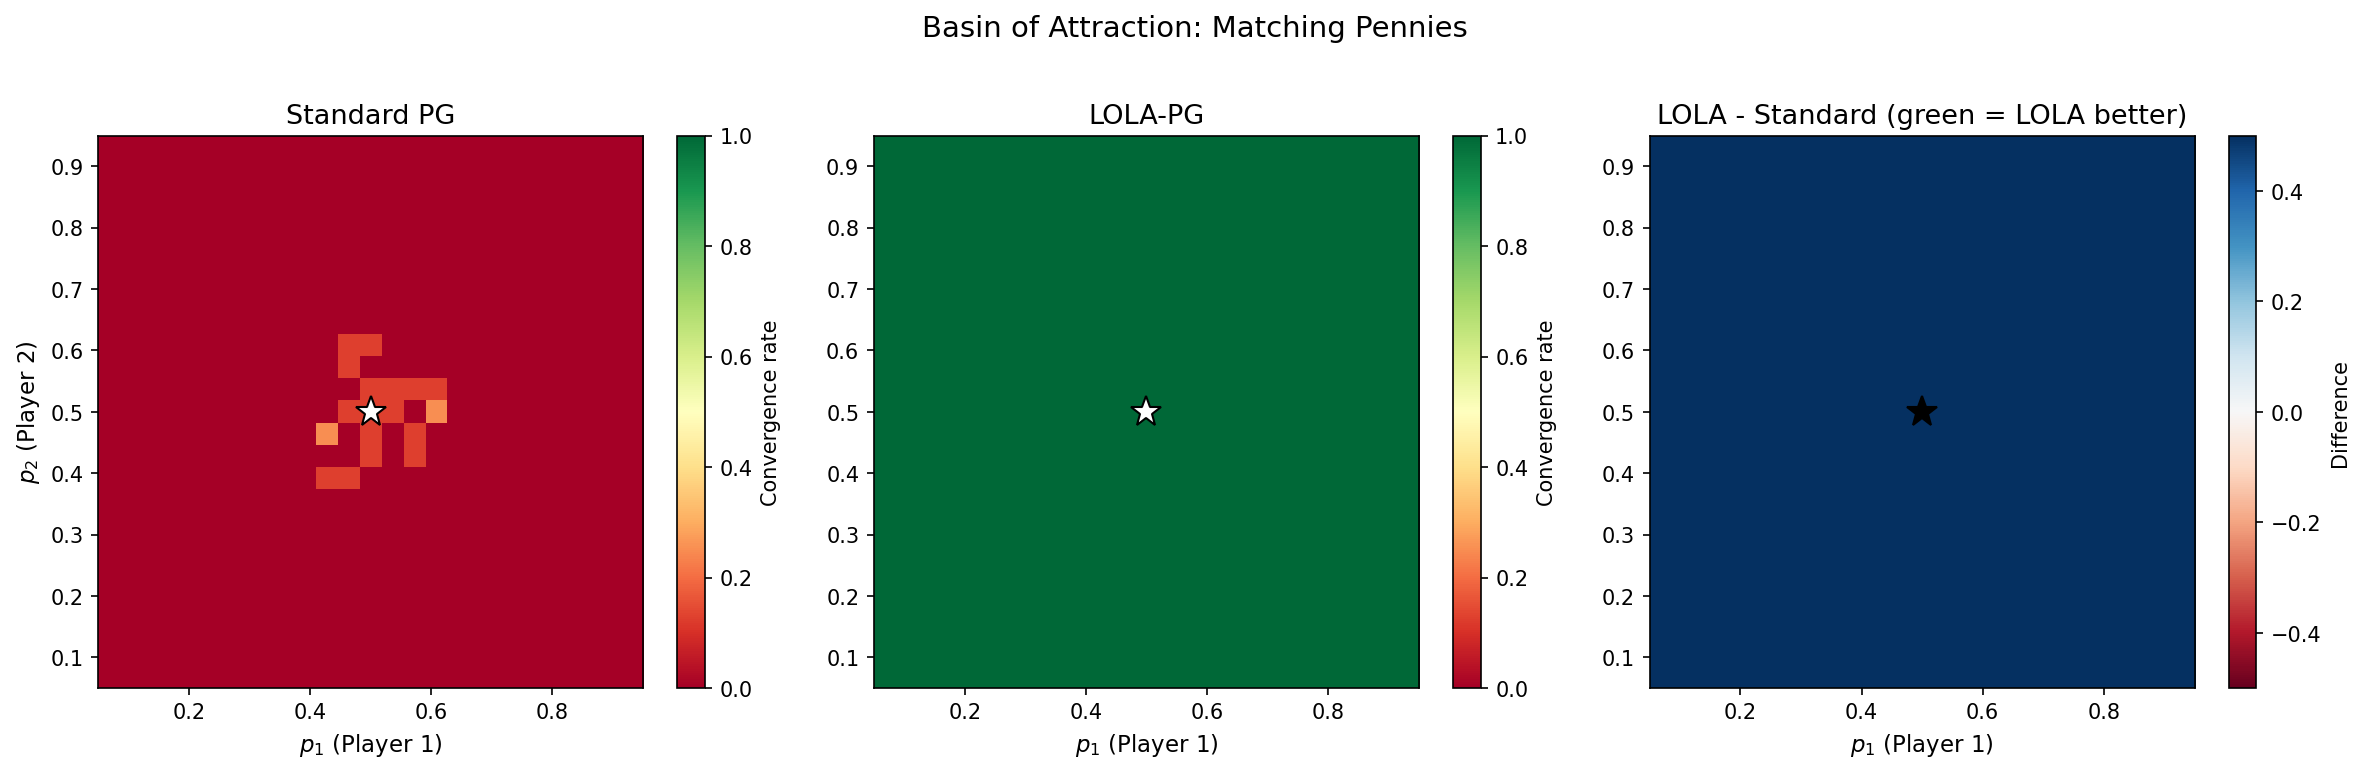
\includegraphics[width=\textwidth]{../figures/basin_matching_pennies.png}
  \caption{Basin enlargement: standard PG vs.\ LOLA-PG.}
  \label{fig:lola-basin}
\end{subfigure}
\hfill
\begin{subfigure}[b]{0.48\textwidth}
  \centering
  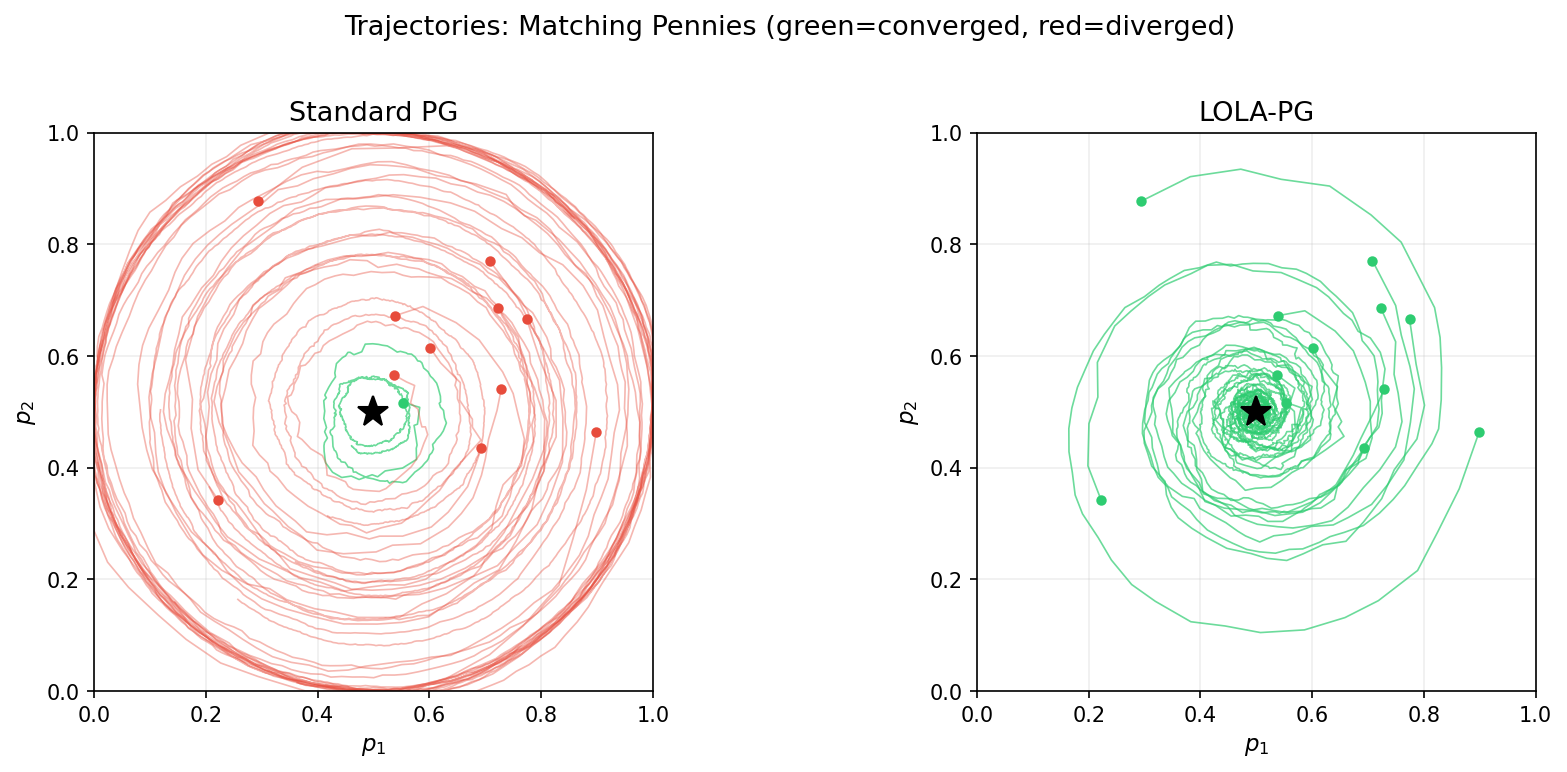
\includegraphics[width=\textwidth]{../figures/trajectories_matching_pennies.png}
  \caption{Trajectories from borderline initialisations.}
  \label{fig:lola-traj}
\end{subfigure}
\caption{LOLA-PG basin enlargement (Matching Pennies, zero-sum).
  Standard PG spirals; LOLA-PG contracts directly to Nash.
  Confirms Theorem~\ref{thm:basin} with $\mu_H > 0$.}
\label{fig:lola}
\end{figure}

%% ═══════════════════════════════════════════════════════════════════════
%%  7. DISCUSSION AND CONCLUSION
%% ═══════════════════════════════════════════════════════════════════════
\section{Discussion and Conclusion}

We have identified two independent levers for improving policy gradient
convergence in general stochastic games:

\vspace{-0.3em}
\begin{itemize}
\item \textbf{Precision weighting} addresses \emph{who} computes the
  gradient: agents with better data should contribute more to the
  update. The gain is quantified exactly by AM-HM inequality on the
  noise variances.
\item \textbf{Opponent shaping} addresses \emph{how} the gradient is
  computed: by anticipating opponents' responses, the effective drift
  field gains an additional contraction term (when the spectral
  reinforcement condition holds).
\end{itemize}
\vspace{-0.3em}

Together, these give a principled, quantified framework for when
and why each technique helps, and when it does not (potential
games, dominance-solvable games). The characterisation via the
opponent-shaping Hessian's spectral properties provides a new
diagnostic tool for practitioners: compute $\mu_H$ to predict
whether LOLA will help.

\paragraph{Limitations.}
The EWPG improvement assumes the precision model $\sigma_i^2 \propto 1/\tau_i$;
misspecification of weights reduces but does not eliminate the benefit.
The spectral reinforcement condition requires computing $H(\pi^*)$,
which is unknown in practice; it can be estimated online from gradient
Jacobians. Extending both results to neural network policies (beyond
tabular) is left for future work.

\paragraph{Open questions for the workshop.}
Is there an optimal joint design of precision weights and LOLA
step-sizes? Can the spectral reinforcement condition be relaxed to
a \emph{probabilistic} analogue (spectral reinforcement in
expectation) to cover stochastic opponent models?

%% ═══════════════════════════════════════════════════════════════════════
%%  REFERENCES
%% ═══════════════════════════════════════════════════════════════════════
\bibliographystyle{plainnat}
\bibliography{../references/references}

\end{document}
